\documentclass{beamer}
\usepackage{graphicx}
\usepackage{tikz}
\usepackage{algorithm}
\usepackage{algpseudocode}


%THEME and COLORTHEME
\usetheme{Madrid}
%\usetheme{Berkeley}
%\usetheme{Copenhagen}

%\usecolortheme{spruce}
%\usecolortheme{beetle}
%\usecolortheme{seahorse}
%\usecolortheme{wolverine}

\title{Hopcroft-Karp Algorithm}

%\subtitle{An Introduction}

\author[Rakib,Sany,Bijoy]{1905047-Rakib Abdullah\\1905048-Md. Al-Amin Sany\\1905052-Bijoy Ahmed Saiem}

\institute[CSE, BUET]
{
Department of Computer Science and Engineering\\
Bangladesh University of Engineering and Technology
}

\date{\today}

%\logo{\includegraphics[height=1cm]{overleaf.png}}

% PLACING ToC AT THE BEGINNING OF EACH SECTION
\AtBeginSection[]
{
\begin{frame}
\frametitle{Table of Contents}
\tableofcontents[currentsection]
\end{frame}
}

\begin{document}

\frame{\titlepage}

%TABLE OF CONTENTS
\begin{frame}
\tableofcontents
\end{frame}

\section{Introduction}
\begin{frame}{Introduction}
\begin{block}{Hopcroft-Karp Algorithm}
The Hopcroft-Karp algorithm is a graph algorithm that finds the maximum cardinality matching in a bipartite graph.
\end{block} \pause
\begin{columns}[T]
\begin{column}{0.5\textwidth}
\centering
\begin{figure}
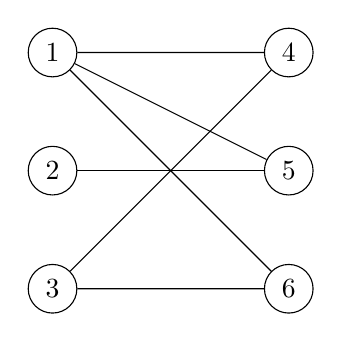
\begin{tikzpicture}[scale=1.5]
  \node[draw, circle] (a1) at (0,1) {1};
  \node[draw, circle] (a2) at (0,0) {2};
  \node[draw, circle] (a3) at (0,-1) {3};
  \node[draw, circle] (b1) at (2,1) {4};
  \node[draw, circle] (b2) at (2,0) {5};
  \node[draw, circle] (b3) at (2,-1) {6};
  
  \draw (a1) -- (b1);
  \draw (a1) -- (b2);
  \draw (a1) -- (b3);
  \draw (a2) -- (b2);
  \draw (a3) -- (b1);
  \draw (a3) -- (b3);
\end{tikzpicture}
\caption{Bipartite graph}
\end{figure}
\end{column}
\pause
\begin{column}{0.5\textwidth}
\centering
\begin{figure}
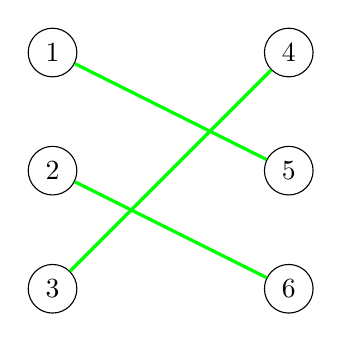
\begin{tikzpicture}[scale=1.5]
  \node[draw, circle] (a1) at (0,1) {1};
  \node[draw, circle] (a2) at (0,0) {2};
  \node[draw, circle] (a3) at (0,-1) {3};
  \node[draw, circle] (b1) at (2,1) {4};
  \node[draw, circle] (b2) at (2,0) {5};
  \node[draw, circle] (b3) at (2,-1) {6};
  
  \draw[green, very thick] (a1) -- (b2);
  \draw[green, very thick] (a2) -- (b3);
  \draw[green, very thick] (a3) -- (b1);
\end{tikzpicture}
\caption{Maximum cardinality matching}
\end{figure}
\end{column}
\end{columns}
\end{frame}

\section{Definitions}
\begin{frame}{Definitions}
     \begin{block}{Bipartite Graph}
A graph is bipartite if its vertices can be divided into two disjoint sets such that every edge connects a vertex in one set to a vertex in the other set.
\end{block}
 \pause
\begin{block}{Maximum Cardinality}
A matching in a graph is a set of edges such that no two edges share a common vertex.Maximum cardinality means maximum possible matching.
\end{block} \pause
\begin{block}{Free vertex}
 A free vertex is a vertex with no matching edge connected to it.
\end{block} \pause

\begin{block}{Augmenting Path}
    \begin{itemize}
        \item Starts and ends both at free vertex
        \item Edges in the path alternate between being in the matching and not in the matching
    \end{itemize}
\end{block}
\end{frame}

\section{Algorithm}
\begin{frame}{Algorithm}
\renewcommand{\thealgorithm}{}
\begin{algorithm}[H]
\floatname{algorithm}{}
\caption{Hopcroft-Karp(G)}
\begin{algorithmic}[1]
\State $M=\phi$ \pause
\Repeat 
\State $P=\{p_1,p_2,\dots,p_k\}$ {\tiny //maximal set of vertex-disjoint shortest augmenting paths} \pause
\State $M:=M\oplus\{p_1 \cup p_2 \cup \dots \cup p_k\}$\pause
\Until{$P=\phi$} \pause
\State Output the matching $M$ as the maximum cardinality matching.
\end{algorithmic}
\end{algorithm}
\end{frame}

\begin{frame}{Example}
A bipartite graph is given below where we will find its maximum cardinality mathching:\\
 \vspace{.5cm}
    \centering
\begin{tikzpicture}[scale=1.5]
\tikzset{vertex/.style = {shape=circle,draw,minimum size=1.5em}}
\tikzset{edge/.style = {->,> = latex'}}

% Left partition
\node[vertex] (A) at (-2,2) {$a$};
\node[vertex] (B) at (-1,2) {$b$};
\node[vertex] (C) at (.5,2) {$c$};
\node[vertex] (D) at (2,2) {$d$};

% Right partition
\node[vertex] (E) at (-2,-1) {$e$};
\node[vertex] (F) at (-1,-1) {$f$};
\node[vertex] (G) at (0,-1) {$g$};
\node[vertex] (H) at (2,-1) {$h$};

% Edges
\draw[edge] (A) to (E);
\draw[edge] (A) to (F);
\draw[edge] (A) to (H);
\draw[edge] (B) to (E);
\draw[edge] (C) to (F);
\draw[edge] (D) to (E);
\draw[edge] (D) to (F);
\draw[edge] (D) to (G);
\draw[edge] (D) to (H);
\end{tikzpicture}
\end{frame}

\begin{frame}{First iteration:BFS}
\only<1>{$\hspace{4.5cm}\text{BFS sources}=\{a,b,c,d\}$}\\ 
\only<2>{$\hspace{4.5cm}\text{BFS sources}=\{\textcolor{red}{a},b,c,d\}$}\\ 
\only<3>{$\hspace{4.5cm}\text{BFS sources}=\{a,\textcolor{red}{b},c,d\}$}\\ 
\only<4>{$\hspace{4.5cm}\text{BFS sources}=\{a,b,\textcolor{red}{c},d\}$}\\ 
\only<5>{$\hspace{4.5cm}\text{BFS sources}=\{a,b,c,\textcolor{red}{d}\}$}\\ 

\only<1>{$\hspace{4.5cm}F=\{\}$}\\ % will only appear on slide 1
\only<2>{$\hspace{4.5cm}F=\{\textcolor{red}{e},\textcolor{red}{f},\textcolor{red}{h}\}$}\\ % will appear on slides 2 and later
\only<3>{$\hspace{4.5cm}F=\{e,f,h\}$}\\
\only<4>{$\hspace{4.5cm}F=\{e,f,h\}$}\\
\only<5>{$\hspace{4.5cm}F=\{e,f,h,\textcolor{red}{g}\}$}\\
\vspace{.5cm}
\hspace{2.7cm}
    \begin{tikzpicture}[scale=1.5]
\tikzset{vertex/.style = {shape=circle,draw,minimum size=1.5em}}
\tikzset{edge/.style = {->,> = latex'}}
\tikzset{red vertex/.style={vertex,fill=red!50}}
\tikzset{blue vertex/.style={vertex,fill=blue!50}}

% Left partition
\node[blue vertex] (A) at (-2,2) {$a$};
\node[blue vertex] (B) at (-1,2) {$b$};
\node[blue vertex] (C) at (.5,2) {$c$};
\node[blue vertex] (D) at (2,2) {$d$};

% Right partition
\node[blue vertex] (E) at (-2,-1) {$e$};
\node[blue vertex] (F) at (-1,-1) {$f$};
\node[blue vertex] (G) at (0,-1) {$g$};
\node[blue vertex] (H) at (2,-1) {$h$};

% Edges
\draw[edge] (A) to (E);
\draw[edge] (A) to (F);
\draw[edge] (A) to (H);
\draw[edge] (B) to (E);
\draw[edge] (C) to (F);
\draw[edge] (D) to (E);
\draw[edge] (D) to (F);
\draw[edge] (D) to (G);
\draw[edge,color] (D) to (H);

% BFS
\onslide<2->{
%\node[blue vertex] (B) at (-2,1) {$b$};
\draw[edge,color=red] (A) to (E);
\draw[edge,color=red] (A) to (F);
\draw[edge,color=red] (A) to (H);
}

\onslide<3->{
\draw[edge,color=red] (B) to (E);
}

\onslide<4->{
\draw[edge,color=red] (C) to (F);
}

\onslide<5->{
\draw[edge,color=red] (D) to (E);
\draw[edge,color=red] (D) to (F);
\draw[edge,color=red] (D) to (G);
\draw[edge,color=red] (D) to (H);
}

\end{tikzpicture} 

\end{frame}


\begin{frame}{First iteration:DFS}
    
    \only<1-2>{$\hspace{4.6cm}F=\{\textcolor{red}{e},f,h,g\}$}\\
    \only<3>{$\hspace{4.6cm}F=\{f,h,g\}$}\\
    \only<1-3>{$\hspace{4.6cm}P=\{\textcolor{red}{(e-a)}\}$}\\
    %\only<1-3>{$\hspace{4.6cm}M=\{\textcolor{red}{(e-a)}\}$}\\
    
    \only<4>{$\hspace{4.6cm}F=\{\textcolor{red}{f},h,g\}$}\\
    \only<4>{$\hspace{4.6cm}P=\{(e-a),\textcolor{red}{(f-c)}\}$}\\
    %\only<4>{$\hspace{4.6cm}M=\{(e-a),\textcolor{red}{(f-c)}\}$}\\
    
    \only<5>{$\hspace{4.6cm}F=\{h,g\}$}\\
    \only<5>{$\hspace{4.6cm}P=\{(e-a),\textcolor{red}{(f-c)}\}$}\\
    %\only<5>{$\hspace{4.6cm}M=\{(e-a),\textcolor{red}{(f-c)}\}$}\\
    
    \only<6>{$\hspace{4.6cm}F=\{h,\textcolor{red}{g}\}$}\\
    \only<6>{$\hspace{4.6cm}P=\{(e-a),(f-c),\textcolor{red}{(g-d)}\}$}\\
    %\only<6>{$\hspace{4.6cm}M=\{(e-a),(f-c),\textcolor{red}{(g-d)}\}$}\\
    
    \only<7>{$\hspace{4.6cm}F=\{h\}$}\\
    \only<7>{$\hspace{4.6cm}P=\{(e-a),(f-c),(g-d)\}$}\\
    \only<7>{$\hspace{4.6cm}\text{Before } M=\phi$}\\
    \only<7>{$\hspace{4.6cm}\text{After }M=M\oplus \{(e-a)\cup(f-c)\cup(g-d)\}$}\\
    \only<7>{$\hspace{4.6cm}M=\{(e-a),(f-c),(g-d)\}$}\\
\vspace{.5cm}
\hspace{2.7cm}
    \begin{tikzpicture}[scale=1.5]
\tikzset{vertex/.style = {shape=circle,draw,minimum size=1.5em}}
\tikzset{edge/.style = {->,> = latex'}}
\tikzset{red vertex/.style={vertex,fill=red!50}}
\tikzset{blue vertex/.style={vertex,fill=blue!50}}


% Left partition
\node[red vertex] (A) at (-2,2) {$a$};
\node[blue vertex] (B) at (-1,2) {$b$};
\node[blue vertex] (C) at (0.5,2) {$c$};
\node[blue vertex] (D) at (2,2) {$d$};

% Right partition
\node[blue vertex] (E) at (-2,-1) {$e$};
\node[blue vertex] (F) at (-1,-1) {$f$};
\node[blue vertex] (G) at (0,-1) {$g$};
\node[blue vertex] (H) at (2,-1) {$h$};

% Edges
\node[red vertex] (E) at (-2,-1) {$e$};
\draw[edge,color=green,line width=1.5pt] (A) to (E);
\draw[edge,color=red] (A) to (F);
\draw[edge,color=red] (A) to (H);
\draw[edge,color=red] (B) to (E);
\draw[edge,color=red] (C) to (F);
\draw[edge,color=red] (D) to (E);
\draw[edge,color=red] (D) to (F);
\draw[edge,color=red] (D) to (G);
\draw[edge,color=red] (D) to (H);

\pause

\draw[edge,color=white,line width=3pt] (A) to (E);

\draw[edge,color=white,line width=3pt] (A) to (F);
\draw[edge,color=white,line width=3pt] (A) to (H);
\draw[edge,color=white,line width=3pt] (B) to (E);
\draw[edge,color=red] (C) to (F);
\draw[edge,color=white,line width=1pt] (D) to (E);
\draw[edge,color=red,line width=1pt] (C) to (F);
\draw[edge,color=red,line width=1pt] (D) to (F);
\draw[edge,color=red,line width=1pt] (D) to (G);
\draw[edge,color=red,line width=1pt] (D) to (H);




\pause
\node[shape=circle,draw=white,minimum size=2em,fill=white] (A) at (-2,2) {};
\node[shape=circle,draw=white,minimum size=2em,fill=white] (A) at ((-2,-1) {};
\node[shape=circle,draw=white,minimum size=2em,fill=white] (A) at (-1,2) {};

\pause  
\draw[edge,color=green,line width=1.5pt] (C) to (F);
\node[red vertex] (F) at (-1,-1) {$f$};
\node[red vertex] (C) at (.5,2) {$c$};

\pause
\draw[edge,color=white,line width=3pt] (C) to (F);
\draw[edge,color=white,line width=3pt] (D) to (F);
\node[shape=circle,draw=white,minimum size=2em,fill=white] (A) at (-1,-1) {};
\node[shape=circle,draw=white,minimum size=2em,fill=white] (A) at (.5,2) {};

\pause
\draw[edge,color=green,line width=1.5pt] (D) to (G);
\node[red vertex] (G) at (0,-1) {$g$};
\node[red vertex] (D) at (2,2) {$d$};

\pause
\draw[edge,color=white,line width=3pt] (D) to (G);
\draw[edge,color=white,line width=3pt] (D) to (H);
\node[shape=circle,draw=white,minimum size=2em,fill=white] (A) at (2,2) {};
\node[shape=circle,draw=white,minimum size=2em,fill=white] (A) at (0,-1) {}; 

\end{tikzpicture}
\end{frame}

\begin{frame}{After first iteration}
After running the DFS, $$M=\{(e-a),(f-c),(g-d)\}$$ \\
\vspace{.35cm}
\hspace{2.7cm}
    \begin{tikzpicture}[scale=1.5]
\tikzset{vertex/.style = {shape=circle,draw,minimum size=1.5em}}
\tikzset{edge/.style = {->,> = latex'}}
\tikzset{red vertex/.style={vertex,fill=red!50}}
\tikzset{blue vertex/.style={vertex,fill=blue!50}}

% Left partition
\node[red vertex] (A) at (-2,2) {$a$};
\node[blue vertex] (B) at (-1,2) {$b$};
\node[red vertex] (C) at (.5,2) {$c$};
\node[red vertex] (D) at (2,2) {$d$};

% Right partition
\node[red vertex] (E) at (-2,-1) {$e$};
\node[red vertex] (F) at (-1,-1) {$f$};
\node[red vertex] (G) at (0,-1) {$g$};
\node[blue vertex] (H) at (2,-1) {$h$};

% Edges
\draw[edge,color=green,line width=1.5pt] (A) to (E);
\draw[edge] (A) to (F);
\draw[edge] (A) to (H);
\draw[edge] (B) to (E);
\draw[edge,color=green,line width=1.5pt] (C) to (F);
\draw[edge] (D) to (E);
\draw[edge] (D) to (F);
\draw[edge,color=green,line width=1.5pt] (D) to (G);
\draw[edge,color] (D) to (H);
\end{tikzpicture}
\end{frame}

\begin{frame}{Second iteration:BFS}
    \only<1-3>{$\hspace{3cm}\text{BFS sources}=\{\textcolor{red}{b}\}$}\\ 

    \only<1-2>{$\hspace{3cm}F=\{\}$} \\
    \only<1>{$\hspace{3cm}\text{BFS tree}=b->e$}
    \only<2>{$\hspace{3cm}\text{BFS tree}=b->e->a$}
    \only<3>{$\hspace{3cm}F=\{\textcolor{red}{h}\}$}\\
    \only<3>{$\hspace{3cm}\text{BFS tree}=b->e->a->f,
    \textcolor{blue}{h}$}\\
    \vspace{.5cm}
\hspace{2.7cm}
    \begin{tikzpicture}[scale=1.5]
\tikzset{vertex/.style = {shape=circle,draw,minimum size=1.5em}}
\tikzset{edge/.style = {->,> = latex'}}
\tikzset{red vertex/.style={vertex,fill=red!50}}
\tikzset{blue vertex/.style={vertex,fill=blue!50}}

% Left partition
\node[red vertex] (A) at (-2,2) {$a$};
\node[blue vertex] (B) at (-1,2) {$b$};
\node[red vertex] (C) at (.5,2) {$c$};
\node[red vertex] (D) at (2,2) {$d$};

% Right partition
\node[red vertex] (E) at (-2,-1) {$e$};
\node[red vertex] (F) at (-1,-1) {$f$};
\node[red vertex] (G) at (0,-1) {$g$};
\node[blue vertex] (H) at (2,-1) {$h$};

% Edges
\draw[edge,color=green,line width=1.5pt] (A) to (E);
\draw[edge] (A) to (F);
\draw[edge] (A) to (H);
\draw[edge,color=red,line width=1.5pt] (B) to (E);
\draw[edge,color=green,line width=1.5pt] (C) to (F);
\draw[edge] (D) to (E);
\draw[edge] (D) to (F);
\draw[edge,color=green,line width=1.5pt] (D) to (G);
\draw[edge,color] (D) to (H);

\pause
\draw[edge,color=blue,line width=1.5pt] (A) to (E);
\pause
\draw[edge,color=red,line width=1.5pt] (A) to (H);
\draw[edge,color=red,line width=1.5pt] (A) to (F);
\end{tikzpicture}
\end{frame}

\begin{frame}{Second iteration:DFS}
    \only<1>{$\hspace{4.6cm}\text{DFS sources}=\{h\}$}\\
    \only<1>{$\hspace{4.6cm}P=\{\}$}\\
    %\only<1>{$\hspace{4.6cm}M=\{(e-a),(f-c),(g-d)\}$}

    \only<2>{$\hspace{4.6cm}\text{DFS sources}=\{h\}$}\\
    \only<2>{$\hspace{4.6cm}P=\{\textcolor{red}{(h-a-}\}$}\\
    %\only<2>{$\hspace{4.6cm}M=\{\textcolor{blue}{(e-a)},(f-c),(g-d)\}$}

    \only<3>{$\hspace{4.6cm}\text{DFS sources}=\{\textcolor{red}{h}\}$}\\
    \only<3>{$\hspace{4.6cm}P=\{\textcolor{red}{(h-a-e-}\}$}\\

    \only<4>{$\hspace{4.6cm}\text{DFS sources}=\{\textcolor{red}{h}\}$}\\
    \only<4>{$\hspace{4.6cm}P=\{\textcolor{red}{(h-a-e-b)}\}$}\\
    %\only<3-4>{$\hspace{4.6cm}M=\{\textcolor{red}{(h-a)},(f-c),(g-d)\}$}

    \only<5>{$\hspace{4.6cm}\text{DFS sources}=\{\}$}\\
    \only<5>{$\hspace{4.6cm}P=\{\textcolor{red}{(h-a-e-b)}\}$}\\
    %\only<5>{$\hspace{4.6cm}M=\{(h-a),(f-c),(g-d)\}$}

    %\only<6>{$\hspace{4.6cm}\text{DFS sources}=\{\}$}\\
    \only<6>{$\hspace{4.6cm}P=\{\textcolor{red}{(h-a-e-b)}\}$}\\
    %\only<6-7>{$\hspace{4.6cm}M=\{\textcolor{red}{(e-b)},(h-a),(f-c),(g-d)\}$}

    %\only<8>{$\hspace{4.6cm}\text{DFS sources}=\{\}$}\\
    %\only<8>{$\hspace{4.6cm}P=\{(h-a),\textcolor{blue}{(a-e)},(e-b)\}$}\\
    %\only<8>{$\hspace{4.6cm}M=\{(e-b),(h-a),(f-c),(g-d)\}$}

    \only<6>{$\hspace{4.6cm}\text{Before } M=\{(a-e),(f-c),(g-d)\}$}\\
    \only<6>{$\hspace{4.6cm}\text{After }M=M\oplus \{(h-a),(a-e),(e-b)\} $}\\
    \only<6>{$\hspace{4.6cm}M=\{(h-a),(e-b),(f-c),(g-d)\}$}\\
    
        \vspace{.5cm}
\hspace{2.7cm}
    \begin{tikzpicture}[scale=1.5]
\tikzset{vertex/.style = {shape=circle,draw,minimum size=1.5em}}
\tikzset{edge/.style = {->,> = latex'}}
\tikzset{red vertex/.style={vertex,fill=red!50}}
\tikzset{blue vertex/.style={vertex,fill=blue!50}}

% Left partition
\node[red vertex] (A) at (3.5,0) {$a$};
\node[blue vertex] (B) at (3.5,2) {$b$};
%\node[red vertex] (C) at (.5,2) {$c$};
%\node[red vertex] (D) at (2,2) {$d$};

% Right partition
\node[red vertex] (E) at (3.5,1) {$e$};
\node[red vertex] (F) at (3,-1) {$f$};
%\node[red vertex] (G) at (0,-1) {$g$};
\node[blue vertex] (H) at (4,-1) {$h$};

% Edges
\draw[edge,color=red,line width=1.5pt] (A) to (E);
\draw[edge,color=red,line width=1.5pt] (A) to (F);
\draw[edge,color=red,line width=1.5pt] (A) to (H);
\draw[edge,color=red,line width=1.5pt] (B) to (E);
%\draw[edge,color=green,line width=1.5pt] (C) to (F);
%\draw[edge] (D) to (E);
%\draw[edge] (D) to (F);
%\draw[edge,color=green,line width=1.5pt] (D) to (G);
%\draw[edge,color] (D) to (H);

\pause
\draw[edge,color=green,line width=1.5pt] (H) to (A);

\pause
    \draw[edge,color=green,line width=1.5pt] (A) to (E);
    \node[red vertex] (H) at (4,-1) {$h$};
    
\pause

%\draw[edge,color=white,line width=3pt] (A) to (H);
%\draw[edge,color=green,line width=1.5pt] (C) to (F);
%\draw[edge] (D) to (F);
%\draw[edge,color=green,line width=1.5pt] (D) to (G);
%\draw[edge,color=white,line width=3pt] (A) to (F);
%\draw[edge,color=white,line width=3pt] (A) to (E);
%\draw[edge] (D) to (E);
\draw[edge,color=green,line width=1.5pt] (B) to (E);
\node[red vertex] (B) at (3.5,2) {$b$};

%\draw[edge,color=white,line width=3pt] (D) to (H);

\pause
\node[shape=circle,draw=white,thick,minimum size=2em,fill=white] (A) at (3.5,0) {};
\node[shape=circle,draw=white,thick,minimum size=2em,fill=white] (H) at (4,-1) {};
\node[shape=circle,draw=white,thick,minimum size=2em,fill=white] (E) at (3.5,1) {};
\node[shape=circle,draw=white,thick,minimum size=2em,fill=white] (B) at (3.5,2) {};

\draw[edge,color=white,line width=3pt] (A) to (E);
\draw[edge,color=white,line width=3pt] (E) to (B);
\draw[edge,color=white,line width=3pt] (H) to (A);

\pause
\node[shape=circle,draw=white,thick,minimum size=2em,fill=white] (F) at (3,-1) {};
\draw[edge,color=white,line width=3pt] (F) to (A);
% \pause
% \node[shape=circle,draw=white,thick,minimum size=2em,fill=white] (H) at (3.5,0) {};
% \draw[edge,color=white,line width=2pt] (A) to (E);
% \draw[edge,color=green,line width=1.5pt] (B) to (E);
% \node[red vertex] (B) at (3.5,2) {$b$};
% %\node[red vertex] (B) at (-2,1) {$b$};

% \pause
% \draw[edge,color=white,line width=3pt] (B) to (E);
% %\draw[edge,color=white,line width=2pt] (D) to (E);
% %\draw[edge,color=green,line width=1.5pt] (C) to (F);

% \pause
% \node[shape=circle,draw=white,thick,minimum size=2em,fill=white] (B) at (3.5,2) {};
% \node[shape=circle,draw=white,thick,minimum size=2em,fill=white] (E) at (3.5,1) {};
\end{tikzpicture}
\end{frame}

\begin{frame}{Algorithm termination}
As no more free vertex is available in upper set,the algorithm terminates and finally we get the following graph with maximum cardinaliy 4 where
    $M=\{(h-a),(e-b),(f-c),(g-d)\}$\\
        \vspace{.8cm}
\hspace{2.7cm}
    \begin{tikzpicture}[scale=1.5]
\tikzset{vertex/.style = {shape=circle,draw,minimum size=1.5em}}
\tikzset{edge/.style = {->,> = latex'}}
\tikzset{red vertex/.style={vertex,fill=red!50}}
\tikzset{blue vertex/.style={vertex,fill=blue!50}}

% Left partition
\node[red vertex] (A) at (-2,2) {$a$};
\node[red vertex] (B) at (-1,2) {$b$};
\node[red vertex] (C) at (.5,2) {$c$};
\node[red vertex] (D) at (2,2) {$d$};

% Right partition
\node[red vertex] (E) at (-2,-1) {$e$};
\node[red vertex] (F) at (-1,-1) {$f$};
\node[red vertex] (G) at (0,-1) {$g$};
\node[red vertex] (H) at (2,-1) {$h$};

% Edges
\draw[edge,color] (A) to (E);
\draw[edge,color] (A) to (F);
\draw[edge,color=green,line width=2.2pt] (A) to (H);
\draw[edge,color=green,line width=2.2pt] (B) to (E);
\draw[edge,color=green,line width=2.2pt] (C) to (F);
\draw[edge] (D) to (E);
\draw[edge] (D) to (F);
\draw[edge,color=green,line width=2.2pt] (D) to (G);
\draw[edge,color] (D) to (H);
\end{tikzpicture}
\end{frame}

\section{Time Complexity}
\begin{frame}{Complexity Analysis}
\renewcommand{\thealgorithm}{}
\begin{algorithm}[H]
\floatname{algorithm}{}
\caption{Hopcroft-Karp(G)}
\begin{algorithmic}[1]
\State $M=\phi$ {\tiny //$O(1)$}
\Repeat 
\State $P=\{p_1,p_2,\dots,p_k\}$ 
\State $M:=M\oplus\{p_1 \cup p_2 \cup \dots \cup p_k\}$
\Until{$P=\phi$}
\State Return M {\tiny //$O(1)$}
\end{algorithmic}
\end{algorithm}
\end{frame}

\begin{frame}{Complexity Analysis}
    \textbf{\small Per Loop Iteration}\\
    \textbf{\small Breadth First Search:}Uses all edges at most once so time complexity is $O(|E|)$\\
    \textbf{\small Depth First Search:}Since vertices and edges are deleted once used,all edges are also used at most once,so time complexity is $O(|E|)$\\
    \textbf{\big So over all each iteration is linear with the number of edges. i.e $O(|E|)$}
\end{frame}

\begin{frame}{Complexity Analysis}
\begin{itemize}
    \item[$\blacktriangle$] Breadth first search terminates when it reaches the free vertex.Therefor,there is no shorter path to a free vertex.Therefore,in subsequent iterations a shorter path cannot be found.\\
    \vspace{.2cm}
    \item[$\blacktriangle$] Once it terminates it collects all free vertex on that level so all possible paths of that length are found.Therefore,in subsequent iterations the paths found must be longer. \\ \\
    \vspace{.2cm}
    \item[$\blacktriangle$] Since the paths alternate between matched and unmatched edges,and free vertices cannot be connected to a matched edge,then in subsequent iterations the paths must be at least two edges longer.\\
\end{itemize}
    
\end{frame}


\begin{frame}{Complexity Analysis}
\begin{itemize}
      \item[$\blacktriangle$]After $\sqrt{|V|}$ iterations the minimum path length would therefore be $2\sqrt{|V|}$\\
    \vspace{.5cm}
     \item[$\blacktriangle$]Since in $P=\{p_1,p_2,\dots,p_k\}$ the paths are vertex disjoint and there are only $|V|$ vertices in the graph,then there can only be $\frac{|V|}{2\sqrt{|V|}}=\frac{1}{2}\sqrt{|V|}$\\ \\
    \vspace{.5cm}
    
    \item[$\blacktriangle$] Therefore after $\sqrt{|V|}$ iterations only $\frac{1}{2}\sqrt{|V|}$ more are needed so the loop will terminate after $\frac{3}{2}\sqrt{|V|}$ repeats.\\
\end{itemize}

\end{frame}

\section{Applications}
\begin{frame}{Applications}
    \begin{itemize}
        \item<1-> \alert{Dating app}-The algorithm can be used in online dating apps to match people based on their interests and preferences.
        \item<2-> \alert{Image segmentation} - finding matches between objects in an image and a pre-defined set of object templates.
        \item<3-> \alert{Job scheduling} - matching workers with tasks based on their skills and availability.
        \item<4-> \alert{Online advertising} - matching ads with potential viewers based on demographic and behavioral data.
    \end{itemize}
\end{frame}





\begin{frame}
\frametitle{Thank You!}
\framesubtitle{Gracias por todo}

\begin{center}
\includegraphics[width=0.7\textwidth]{madrid_logo.jpeg}
\end{center}

\begin{itemize}
\item Thank you for your attention.
\item We appreciate your support.
\end{itemize}


\end{frame}

\end{document}